\documentclass[a4paper]{article}

\usepackage{INTERSPEECH2021}
\usepackage[table]{xcolor}
\usepackage{amsmath}

\title{Final NLU project template}
\name{Edoardo Maines (232226)}

\address{
  University of Trento}
\email{edoardo.maines@studenti.unitn.it}

\begin{document}

\maketitle


\begin{abstract}
This is the report of the project developed for the course Natural Language Understanding (NLU) at the University of Trento. The main goal, in this paper, was to develop a word-level language model using an recurrent neural network (RNN) in order to predict the next word given an input sentence. Regularization techniques have been applied to observe differences in performance, in terms of perplexity with models without such techniques.
\end{abstract}
\section{Introduction (approx. 100 words)} 
The aim of the project is to create a linguistic model using a neural network in order to achieve the goal of having a perplexity of less than 90.7 on the "Penn Treebank Dataset" \cite{marcus-etal-ptb}.\\
So initially the database was downloaded and analyzed. We will see the results of these analyzes in detail later. After doing this, you have to select the model to implement as a baseline: in my case I chose a model with double LSTM layer as RNN model.
To achieve the goal, two main regularization techniques have been implemented: naive dropout \cite{zaremba-rnn}  and Variational Dropout \cite{gal-dropout}.\\
    

\section{Task Formalisation (approx. 200 words)}

Language modeling is a subfield of Natural Language Processing (NLP) that primarily focuses on predicting the next word. Of course, this is not the only area in which it is applied: in fact, language modeling is found applied in the main techniques for solving natural language understanding problems, such as machine translation, speech synthesis, and text classification.
A language model is trained on an extremely large dataset so that it can learn the statistical properties of the language used in that specific dataset.
The goal of language modeling is to learn a model M that is able to predict the probability of a word w at position p in a sentence of X words:
\[P(w_p|w_1, w_2, ..., w_{x-1}) = M(w_p|w_1, w_2, ..., w_{x-1})\]
In terms of architecture, language modeling allows for the implementation of different types of architectures. Among the main ones and also among those recommended by the professor, we find the basic RNN and the LSTM: RNNs are able to handle sequences of variable-length data, while LSTMs are particularly effective in handling long-term dependency problems.
As mentioned earlier, for this project, an LSTM was chosen as the reference architecture.

\section{Data Description & Analysis (approx. 200-500 words)}
For this project, the "Penn TreeBank Dataset" was used as the dataset. The corpus was directly retrieved from the PyTorch-NLP \cite{pytorch-nlp} which is a library built on PyTorch and entirely devoted to deal with NLP tasks.
Using PyTorch-NLP, the dataset is already split into train, validation and test sets with the following distribution: 85.6\% in train, 6.8\% in validation, and 7.6\% in test.
\newcolumntype{g}{>{\columncolor{lightgray}}c}
\begin{table}[t!]
    \centering
        \begin{tabular}{|g|c|c|c|}
        \hline
        \rowcolor{lightgray} Dataset & \#Sentences & Vocabulary Size & \#Words\\
        \hline
        \rowcolor{gray} \multicolumn{4}{|c|}{Dataset with \textit{\textless /s\textgreater}, \textit{\textless unk\textgreater} and \textit{N} symbols} \\
        \hline
        Train & 42068 & 10000 & 929589 \\
        \hline
        Validation & 3370 & 6022 & 73760\\
        \hline
        Test & 3761 & 6049 & 82430\\
        \hline
        \rowcolor{gray} \multicolumn{4}{|c|}{Dataset with \textit{\textless unk\textgreater} and \textit{N} symbols} \\
        \hline
        Train & 42068 & 9999 & 887521 \\
        \hline
        Validation &  3370 & 6021 & 70390\\
        \hline
        Test & 3761 & 6048 & 78669\\
        \hline
        \rowcolor{gray} \multicolumn{4}{|c|}{Dataset without \textit{\textless /s\textgreater}, \textit{\textless unk\textgreater} and \textit{N} symbols} \\
        \hline
        Train & 42068 & 9997 & 810020 \\
        \hline
        Validation & 3370 & 6019 & 64302\\
        \hline
        Test & 3761 & 6046 & 71352\\
        \hline
        \end{tabular}
    \caption{In this table it is possible to observe, for each dataset, the number of sentences, the size of the vocabulary and the number of words. Furthermore, this analysis is carried out taking into account or not some symbols, \textit{\textless /s\textgreater}, \textit{\textless unk\textgreater} and \textit{N}.}
    \label{tab: vocabolary_analysis}
\end{table}
\begin{table}[t]
        \centering
        \begin{tabular}{|c|c|c|c|}
            \hline
            Dataset & MIN & MAX & AVG\\
            \hline
            Train & 1 & 82 & 21\\
            \hline
            Validation & 1 & 74 & 21\\
            \hline
            Test & 1 & 77 & 21\\
            \hline
        \end{tabular}
        \caption{this table shows, for each dataset, different analyzes carried out on the sentences. Indeed, we find the minimum length (MIN), the maximum length (MAX) and the average length (AVG).}
        \label{tab: sentences_analysis}
\end{table}
\\
Once the database corpus was obtained, several analyzes were performed to observe the structure of this dataset and these analyzes are shown in Table \ref{tab: vocabolary_analysis}, Table \ref{tab: sentences_analysis} and Table \ref{tab: frequencies}.
\\
The dataset is already heavily pre-processed and for this reason, within each dataset, we find various symbols and tags: every number has been replaced by \textit{N} and every word outside the dictionary by \textit{\textless unk\textgreater}. Moreover, while loading the dataset, the tag \textit{\textless /s\textgreater} is added to the end of each sentence.
So, to observe the variations due to the presence of these symbols, I have carried out several analyses, with and without symbols. In each table, data is presented both for analyses taking into account symbols and also for analyses where symbols are not considered.
\\
In Table \ref{tab: vocabolary_analysis}, for each dataset, the number of sentences, the vocabulary size, and the number of words are reported respectively. Looking at the data reported in Table 1, it can be observed that the validation and test sets are respectively 7.9\% and 8.9\% of the training set, and contain the majority of the words in the dictionary. In fact, when compared to the training set, the validation set has 60.2\% of the words, while the test set has 60.5\%. It should be noted that, even when taking into account symbols or not, the number of sentences does not change since the presence or absence of symbols does not affect the result in any way.
\\
Table \ref{tab: sentences_analysis}, on the other hand, shows some statistics related to the sentences within the three datasets. The first data found is the minimum length of sentences, then we have the maximum length and finally, the average length. It should be noted that, in this case, they behave consistently across the different datasets.
\\
As already mentioned earlier, the pre-processing was already performed by the authors: in fact, the text is already in lowercase, numbers have been replaced with the value N, punctuation has been removed, and infrequent words have been replaced with \textit{\textless unk\textgreater}. Given the presence of these latter tags, the vocabulary is represented by the 10000 most frequent words. So, in Table \ref{tab: frequencies}, we find the list of the 10 most frequent words within the entire corpus.
\\
\begin{table}[h]
    \begin{minipage}{.5\linewidth}
     
        \centering
        \begin{tabular}{|c|c|c|}
            \hline
            Rank & Freq & Word\\
            \hline
            1 & 59421 & the\\
            \hline
            2 & 53299 & \textless unk\textgreater\\
            \hline
            3 & 37607 & N\\
            \hline
            4 & 28427 & of\\
            \hline
            5 & 27430 & to\\
            \hline
            6 & 24755 & a\\
            \hline
            7 & 21032 & in\\
            \hline
            8 & 20404 & and\\
            \hline
            9 & 11555 & 's\\
            \hline
            10 & 10436 & for\\
            \hline
        \end{tabular}
        \caption{}
        \label{freq_1}
    \end{minipage}%
    \begin{minipage}{.5\linewidth}
        \centering  
        \begin{tabular}{|c|c|c|}
            \hline
            Rank & Freq & Word\\
            \hline
            1 & 59421 & the\\
            \hline
            2 & 28427 & of\\
            \hline
            3 & 27430 & to\\
            \hline
            4 & 24755 & a\\
            \hline
            5 & 21032 & in\\
            \hline
            6 & 20404 & and\\
            \hline
            7 & 11555 & 's\\
            \hline
            8 & 10436 & for\\
            \hline
            9 & 10419 & that\\
            \hline
            10 & 8764 & \$\\
            \hline
        \end{tabular}
        \caption{}
        \label{freq_2}
    \end{minipage} 
    \caption{10 most frequent words. As shown in Table \ref{freq_1}, we take into account the symbols N and \textless unk\textgreater, while in Table \ref{freq_2} these symbols have been removed.}
    \label{tab: frequencies}
\end{table}
\\
\section{Model (approx. 200-500 words)}
As mentioned earlier, for the implementation of this project, I took as a reference the work done by \textit{Zaremba et al.} \cite{zaremba-rnn} more specifically, as a baseline, I created an unregularized LSTM architecture and then a medium and highly regularized LSTM with naive dropout. As mentioned in the above paper \cite{zaremba-rnn}, dropout, the most successful technique for regularization neural networks, does not work well with RNNs, and so also with LSTMs. In fact, in order to reduce overfitting, naive dropout can be applied only on the non-recurrent connections, as shown in Figure \ref{fig:naive-variational}.
\\
The structure used as a baseline is very simple: it consists of an embedding layer, followed by two LSTM layers, and finally a dense layer to restore the initial dimensions.
\\
Subsequently, for the regularized architectures, I applied a dropout layer before and after the LSTM layers. However, dropout was also applied to the output of the LSTM layers, to be specific, on the non-recurrent connections.
\\
Let's see now how to mathematically represent our multi-layer LSTM structure:

\begin{equation}
\begin{align*}
&i_t = \sigma(W_{ii}h_{t}^{l-1} + b_{ii} + W_{hi}h_{t-1}^{l} + b_{hi})\\
&f_t = \sigma(W_{if}h_{t}^{l-1} + b_{if} + W_{hf}h_{t-1}^{l} + b_{hf})\\
&g_t = \tanh(W_{ig}h_{t}^{l-1} + b_{ig} + W_{hg}h_{t-1}^{l} + b_{hg})\\
&o_t = \sigma(W_{io}h_{t}^{l-1} + b_{io} + W_{ho}h_{t-1}^{l} + b_{ho})\\
&c_t^l = f_{t} \odot c_{t-1}^{l} + i_t \odot g_t\\
&h_t^l = o_t \odot \tanh(c_t^l)\\
\end{align*}
\label{lstm_structure}
\end{equation}

where \textit{l} represents the number of LSTM layers at time step \textit{t}. \textit{c\textsubscript{t}}  is the memory cell, \textit{h\textsubscript{l-1}} is the input coming from the previous layer \textit{l-1} at time step \textit{t}, \textit{h\textsubscript{t-1}} represents the hidden state of the layer at time step \textit{t-1}. Finally, \textit{i\textsubscript{t}}, \textit{f\textsubscript{t}}, \textit{g\textsubscript{t}}, and \textit{o\textsubscript{t}} are, respectively, the input, forget, cell and output gates. $\sigma$  represents the sigmoid function and $\odot$ represents element-wise multiplication.
    
\subsection{Naive Dropout}
So, the regularization technique chosen is the \textit{naive dropout} \cite{zaremba-rnn}. This is a technique, very popular with neural networks, which applies a random mask to the units of the network during the training phase. However, as mentioned earlier, this dropout results in a 'counter-productive' action. In fact, for this reason, only non-recurrent connections are affected by the application of the dropout operator \textit{D}, resulting in:    
\begin{equation}
    \begin{align*}
    &i_t = \sigma(W_{ii}\textbf{\textcolor{red}{D}}(h_{t}^{l-1}) + b_{ii} + W_{hi}h_{t-1}^{l} + b_{hi})\\
    &f_t = \sigma(W_{if}\textbf{\textcolor{red}{D}}(h_{t}^{l-1}) + b_{if} + W_{hf}h_{t-1}^{l} + b_{hf})\\
    &g_t = \tanh(W_{ig}\textbf{\textcolor{red}{D}}(h_{t}^{l-1}) + b_{ig} + W_{hg}h_{t-1}^{l} + b_{hg})\\
    &o_t = \sigma(W_{io}\textbf{\textcolor{red}{D}}(h_{t}^{l-1}) + b_{io} + W_{ho}h_{t-1}^{l} + b_{ho})\\
    &c_t^l = f_{t} \odot c_{t-1}^{l} + i_t \odot g_t\\
    &h_t^l = o_t \odot \tanh(c_t^l)\\
    \end{align*}
\label{naive_dropout}
\end{equation}

\subsection{Variational Dropout}
However, there are different techniques of dropout. In fact, in the work done by 'Gal et al.'\cite{gal-dropout}, a variant of the naive dropout \cite{zaremba-rnn} previously applied is presented. This technique is called \textit{Variational Dropout}. They studied the intersection between Bayesian research and deep learning, offering a new point of view and theoretical ground to apply dropout to recurrent connections too.
This approach, therefore, applies the same dropout mask, at each time step, to inputs, outputs, and recurrent layers, and implies the dropping of the same units of the network at each time step.
\\
To better understand the formulation and application of this technique, let's re-parametrise (\ref{naive_dropout}) seen earlier:
\begin{equation}
\Biggl(
\begin{array}{cc}
     \textbf{i}\\\textbf{f}\\\textbf{o}\\\textbf{g}\\
\end{array}
\Biggl) = 
\Biggl(
\begin{array}{cc}
     \sigma\\\sigma\\\sigma\\\tanh\\
\end{array}
\Biggl)
\biggl(
\biggl(
\begin{array}{cc}
     \textbf{h}_{t}^{l-1}\circ z_{x}\\\textbf{h}_{t-1}^{l} \circ z_{h}\\
\end{array}
\biggl) \cdot \textbf{W}
\biggl)
\label{variational_dropout} 
\end{equation}
where \textit{z\textsubscript{x}} and \textit{z\textsubscript{h}} are the repeated random masks at each time step.\\
It should be noted that, in (\ref{variational_dropout}), the dropout operator is not time-dependent, as opposed to (\ref{naive_dropout}). This is because \textit{Zaremba et al.} \cite{zaremba-rnn} apply a new mask at each time step, while in this case, the same mask is always applied.
\\
As shown in Figure \ref{fig:naive-variational} \cite{gal-dropout}, In this depiction squares represent RNN units, vertical arrows represent non-recurrent connections and horizontal arrows represent the recurrent ones. Colored arrows are the ones onto which dropout is applied and different colors represent different dropout masks. As we can see, in (a) different masks are used at different time steps and only non-recurrent connections are affected. In (b), the variational dropout proposal, the same dropout mask is applied at each time step, including onto the recurrent connections.

\begin{figure}
    \centering     
    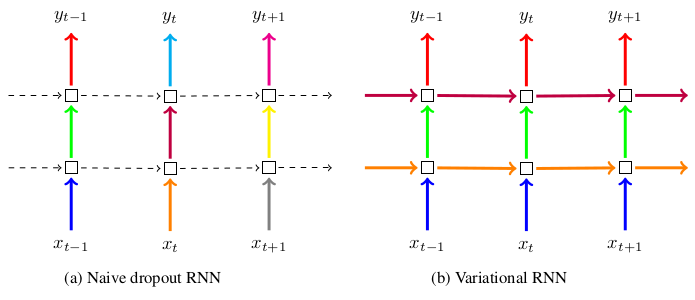
\includegraphics[width=0.45\textwidth]{naive-variational scheme.png}     
    \caption{Image taken from the paper by \textit{Gal et al.} .\cite{gal-dropout}}
    \\
    It shows the differences between the approach by \textit{Zaremba et al.} (a) \cite{zaremba-rnn} and the approach by \textit{Gal et al.} (b) \cite{gal-dropout}
\label{fig:naive-variational}
\end{figure}

\subsection{Practical Experiments}
Thanks to the functionality offered by the Pytorch-NLP library, the database preparation process was particularly easy and fast. In the case of the baseline, the two LSTM layers are unrolled for 20 steps, while, in the case of the regularized, 35 steps. Also, for each architecture, a minibatch length of 20 was chosen.
\\
Let's now look in detail at the two cases: 
\begin{enumerate}
    \item non-regularized:
    \begin{itemize}
        \item baseline [\textit{Zaremba et al.}].
    \end{itemize}
    \item regularized:
    \begin{itemize}
        \item medium-regularizate [\textit{Zaremba et al.}];
        \item high-regularizate [\textit{Zaremba et al.}];
        \item medium-regularizate with Variational Dropout [\textit{Gal et al.}].
    \end{itemize}
\end{enumerate}
Due to the lack of regularization, the size of the non-regularized network cannot be high as this can lead to overfitting.
\\
To prevent this problem, the LSTM layers were made with 200 units each and their weights were initialized uniformly to [-0.1, 0.1]. Additionally, the norm of gradients is clipped at 5. For this model, the training phase ran for 13 epochs with an initial learning rate of 1, which after the fourth epoch, it was decremented by a factor of 2 for each epoch.
\\
In the case of the medium regularized LSTM, each LSTM layer was made with 650 units and their weights were initialized uniformly to [-0.5, 0.5]. Also in this case the norm of gradients is clipped at 5 but, the training phase was composed, instead, by 39 epochs. The learning rate initially 1, after the sixth epoch, is reduced at each epoch by a factor of 1.2. A dropout of 50\% is applied to every non-recurrent connection.
\\
Still using this structure, I tried to apply the Variational Dropout \cite{gal-dropout}, applying different dropout masks in different points of the neural network. More in detail, I applied a dropout mask of 50\% to the embeddings but also to the last outputs of the two LSTM layers. Furthermore, I applied two different dropout masks of 30\% on the recurrent connections of the two LSTM layers and a dropout mask of 40\% on the inputs/outputs in between the two LSTM layers.
\\
Finally, we have the large regularized model. Each layer is made of 1500 units and their weights are initialized uniformly to [-0.04, 0.04]. This time, the norm of gradients is clipped at 10 and the training phase is performed for a total of 55 epochs. As in every case seen before, the initial learning rate is set to 1 but, after the 14th epoch, it is reduced at every epoch by a factor of 1.15. In this case, a dropout of 65\% is applied on the non-recurrent connections.
\\
In conclusion, I used an optimizer (SGD) with a momentum of 0.8 and the loss was calculated using Cross-Entropy.
\\
The initial idea was to perform the training phase 5 times for each structure. However, due to the high computational cost, the training of the largest network was only performed once. To conclude, the mean and standard deviation of the perplexity is calculated and reported. 

\section{Evaluation (approx. 400-800 words)}
\subsection{Perplexity Performance}
As previously mentioned, the metric I selected for evaluation was perplexity. Therefore, to evaluate the efficiency of the regularized models, I used the perplexity of the baseline as a comparison (non-regularized model).
\\
In detail, perplexity was computed using Cross-Entropy:
\begin{equation}
PP(W) = 2^{H(W)} = 2^{-{1\over N}\log_{2}{P(w_1, w_2, ..., w_N)}}
\label{cross_entropy}
\end{equation}
where \textit{PP(W)} represents the perplexity of a sequence of words \textit{W} and \textit{H(W)} the cross-entropy on the same sequence \textit{W}.
The calculation of the final perplexity, calculated on the testing set, can be summarized in 3 main steps:   
\begin{enumerate}
    \item I multiply the perplexity of the batch with the current batch size at each step;
    \item I sum the perplexities of each batch;
    \item I divide the result by the total number of words.
\end{enumerate}
Let's look at the results obtained during the various training phases: I remember that, as mentioned earlier, for all models, with the exception of the largest one, 5 training runs were performed.   
\\
Regarding the non-regularized model, after the 5 training runs, the average perplexity was found to be 124.87 with a standard deviation of 0.076. Regarding, instead, the medium-regularized model, after the training runs, the average perplexity was found to be 93.54 with a standard deviation of 0.035. Thanks to the application of naive dropout, we have a gain in perplexity of 31.33.
\\
The large-regularized model was trained only once due to the high computational power required. The resulting perplexity after a single training was 91.87, thus resulting in a gain in perplexity of 33.
\\
Finally, we have the medium-regularized model to which 'Variational Dropout' \cite{gal-dropout} was applied. After the 5 training runs, the average perplexity was found to be 84.37 with a standard deviation of 0.042.
\\
As we can see from the results reported in Table \ref{tab: ppl_results}, this last model, thanks to the application of 'Variational Dropout', turned out to be the most performing.
\\
\begin{table}[h]
        \centering
        \begin{tabular}{|c|c|}
            \hline
            MODELS & PP(W) on Test Set\\
            \hline
            non-regularized LSTM & 124.87 $\pm$ 0.076\\
            \hline
            Medium regularized LSTM & 93.54 $\pm$ 0.035\\
            \hline
            Large regularized LSTM & 91.87\\
            \hline
            Variational medium LSTM & 84.37 $\pm$ 0.042\\
            \hline
        \end{tabular}
        \caption{This table shows the results, for each model, of the resulting perplexity. It should be noted, however, that as already mentioned, only for the large model more runs were not performed and therefore the resulting perplexity is not an average.}
        \label{tab: ppl_results}
\end{table}
\\
\subsection{Text Generation Test and Example}
In this section, I will show you the experiments I performed with the various trained models and the predicted results. I used the models to predict the next 10 words starting from the following sentence \textit{'The meaning of life is'}.
\\
However, some clarifications are needed before moving on to the results. During the prediction phase, I forced the model not to give as the next word: \textit{\textless unk\textgreater}, \textit{N} and \textit{\$}. Also, in case the token \textit{\textless /s\textgreater} is predicted, the result would be a period (\textit{"."}).
\\
Furthermore, during the prediction phase, I did not select the word with the highest probability but randomly selected, for each word, a word from the vocabulary with a weight corresponding to the probability of being the next one. I thought of this approach because it seemed to me the most realistic.
\\
\\
\textbf{Non-regularized model}
\\
\textit{The meaning of life is there are not a rapid scene and consumers intend to}
\\
\textbf{Medium-Regularized model}
\\
\textit{The meaning of life is not all as intense as the federation of the no.}
\\
\textbf{Large-Regularized model}
\\
\textit{The meaning of life is sold in speeds at a new suggestion called even more}
\\    
\textbf{Variational Medium model}
\\
\textit{The meaning of life is stiff for the other types of discipline and the otherwise}
\\
\\
It should be noted that, using models with different perplexities, the results are also different. In fact, models with higher perplexity values, such as the Non-Regularized model, lead to results that reflect reality worse. On the other hand, using models with lower perplexity, the results are always more consistent.

\section{Conclusion}
The project presented compares different types of dropout applied to the \textit{Penn Treebank dataset} \cite{marcus-etal-ptb}. To make this comparison, a simple model was implemented as a baseline, and then various dropout techniques were applied. The ideas behind these techniques were based on the works by \textit{Zaremba et al.} \cite{zaremba-rnn} and by \textit{Gal et al.} \cite{gal-dropout}.
\\
In summary, for the model used as a baseline, no dropout was applied. For the second and third models (Medium and Large-Regularized), the same dropout technique (naive dropout) was applied but with different sizes. And finally, for the last model, the variational dropout technique was applied.
\\
As shown by the results regarding perplexity in table \ref{tab: ppl_results} and the prediction results in paragraph 5, the best model was found to be the Medium-Regularized with Variational Dropout.
\\
Furthermore, as we can observe from the results, by applying Variational dropout we are able to surpass the perplexity given as the objective.

\bibliographystyle{IEEEtran}

\bibliography{mybib}

 %\begin{thebibliography}{9}
 %\bibitem[1]{Davis80-COP}
 % S.\ B.\ Davis and P.\ Mermelstein,
 %``Comparison of parametric representation for monosyllabic word recognition in %continuously spoken sentences,''
   %\textit{IEEE Transactions on Acoustics, Speech and Signal Processing}, vol.~28, %no.~4, pp.~357--366, 1980.
 %\bibitem[2]{Rabiner89-ATO}
   %L.\ R.\ Rabiner,
   %``A tutorial on hidden Markov models and selected applications in speech %recognition,''
  % \textit{Proceedings of the IEEE}, vol.~77, no.~2, pp.~257-286, 1989.
 %\bibitem[3]{Hastie09-TEO}
   %T.\ Hastie, R.\ Tibshirani, and J.\ Friedman,
   %\textit{The Elements of Statistical Learning -- Data Mining, Inference, and %Prediction}.
   %New York: Springer, 2009.
 %\bibitem[4]{YourName17-XXX}
  % F.\ Lastname1, F.\ Lastname2, and F.\ Lastname3,
   %``Title of your INTERSPEECH 2021 publication,''
   %in \textit{Interspeech 2021 -- 20\textsuperscript{th} Annual Conference of the %International Speech Communication Association, September 15-19, Graz, Austria, %Proceedings, Proceedings}, 2020, pp.~100--104.
% \end{thebibliography}

\end{document}
